% Generated by build_report.py; shared presentation content.
\section{Kiến trúc mô hình BR-Dummy: Geo-I, mạng đường và các cơ chế}
\textbf{Geo-I tạo neo riêng tư từ GPS.} Lịch sử neo + mạng đường + POI công khai tạo tập dummy. Server thấy query; thiết bị giữ GPS để xếp hạng kết quả cuối.

\begin{center}
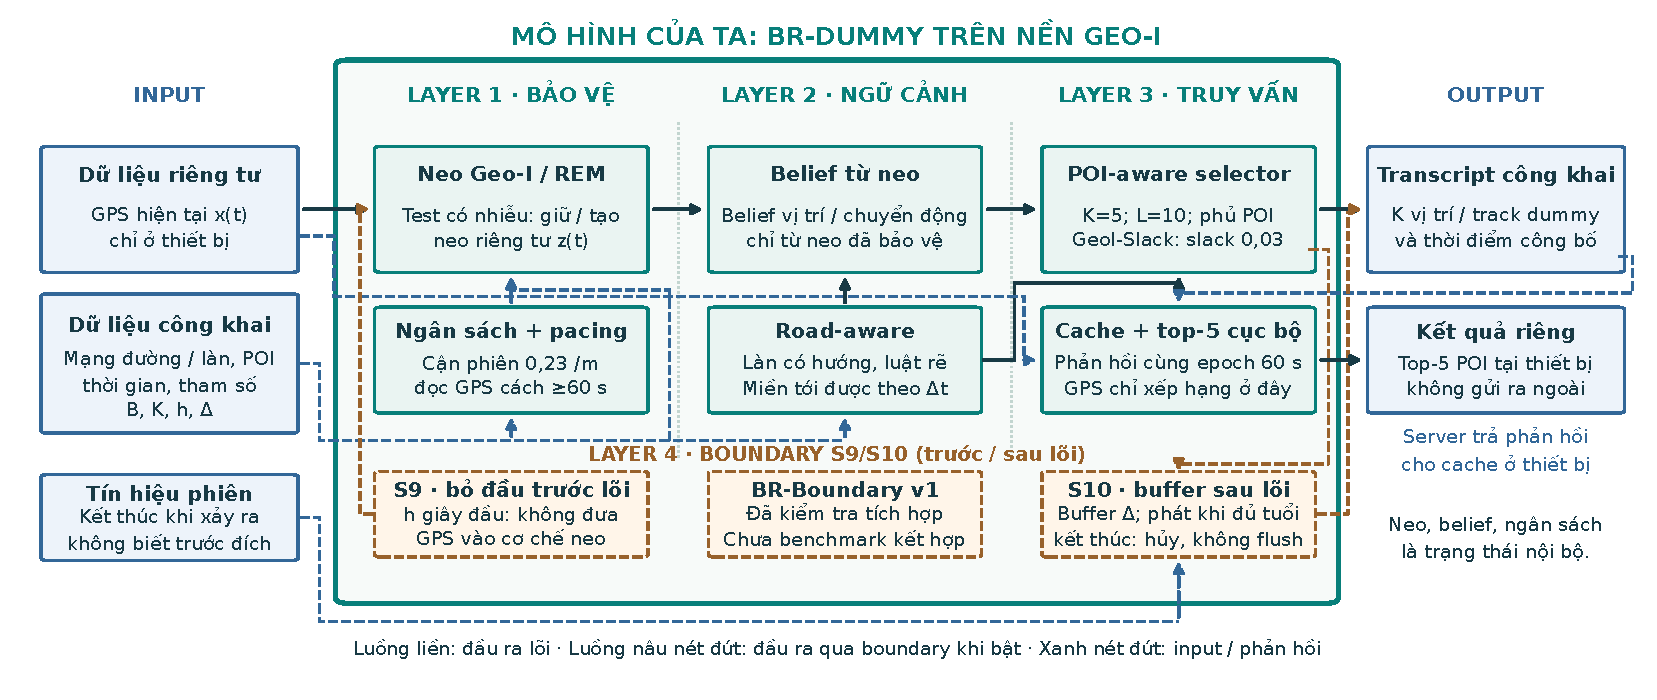
\includegraphics[width=\linewidth]{figures/architecture_model.pdf}
\end{center}
Khung xanh là mô hình. Output công khai: K điểm dummy và thời điểm phát. Output riêng: top-5 POI tại thiết bị.

\begingroup\small
\begin{longtable}{@{}P{5.006cm}P{11.913cm}@{}}
\toprule
\textbf{Component} & \textbf{Vai trò trọng tâm}\\\midrule
\endfirsthead
\toprule
\textbf{Component} & \textbf{Vai trò trọng tâm}\\\midrule
\endhead
\bottomrule\endfoot
Geo-I / REM — S1 & Tạo neo bằng cơ chế nhiễu xác suất; bảo vệ tọa độ từng lần đọc.\\
\addlinespace[3pt]
Tái dùng + ngân sách + pacing — S2/S3 & Giảm nhiều mẫu độc lập khi dừng; giới hạn rò rỉ qua chuỗi; giãn đọc GPS.\\
\addlinespace[3pt]
Belief + road-aware — S3 & Ước lượng vị trí từ neo đã bảo vệ; dummy đi được theo hướng làn và luật rẽ.\\
\addlinespace[3pt]
POI-aware + cache — dịch vụ & Chọn tập dummy phủ POI bổ sung nhau; hợp phản hồi còn hiệu lực, chọn top-5 cục bộ.\\
\addlinespace[3pt]
Boundary — S9/S10 & S9 bỏ đầu trước lõi; S10 buffer sau lõi, hủy phần chưa phát khi chuyến kết thúc.\\
\end{longtable}
\endgroup
Bộ chọn dummy chỉ dùng neo đã bảo vệ và dữ liệu công khai. K dummy không tự tạo k-anonymity. Boundary đã kiểm tra tích hợp, chưa benchmark kết hợp với dịch vụ.

\subsection{Định lượng hai cấu hình Geo-I}
\textbf{GeoI-Paced:} cấu hình đối chứng nội bộ. \textbf{GeoI-Slack:} bản hiện tại, thêm độ linh hoạt khi chọn dummy. Hai bản cùng ngân sách riêng tư và cùng dịch vụ.

\begingroup\small
\begin{longtable}{@{}P{3.938cm}P{6.350cm}P{6.350cm}@{}}
\toprule
\textbf{Tham số / component} & \textbf{GeoI-Paced} & \textbf{GeoI-Slack}\\\midrule
\endfirsthead
\toprule
\textbf{Tham số / component} & \textbf{GeoI-Paced} & \textbf{GeoI-Slack}\\\midrule
\endhead
\bottomrule\endfoot
Neo / ngân sách & $\varepsilon$\_\allowbreak{}test = $\varepsilon$\_\allowbreak{}release = 0,01 /m; θ = 200 m; cận phiên 0,23 /m & Giống GeoI-Paced\\
\addlinespace[3pt]
Đọc GPS / cache & Đọc cách $\ge$60 giây; cache cùng epoch 60 giây & Giống GeoI-Paced\\
\addlinespace[3pt]
Dịch vụ & K=5 điểm; L=10 POI/loại/điểm; chọn top-5 tại thiết bị & Giống GeoI-Paced\\
\addlinespace[3pt]
Slack & Không nới điểm mục tiêu của bộ chọn & Cho phép giảm tối đa 0,03 điểm mục tiêu để di chuyển hữu ích hơn; không phải giảm Recall 3\%\\
\end{longtable}
\endgroup
\key{Đóng góp: phối hợp lịch sử Geo-I đã bảo vệ, ngân sách, mạng làn và mục tiêu phủ POI. Geo-I + dummy đã có tiền lệ [\href{https://wrap.warwick.ac.uk/id/eprint/183198/1/WRAP-privacy-preserving-querying-mechanism-high-utility-electric-vehicles-2024.pdf}{R12}]; lợi ích của cách phối hợp phải được kiểm tra bằng benchmark.}

